\documentclass[margin,line]{resume}
\usepackage[hidelinks]{hyperref}
\usepackage{tikz}
\usepackage{enumitem}
\setlength{\textheight}{9.7in}
\newenvironment{absolutelynopagebreak}
{\par\nobreak\vfil\penalty0\vfilneg
\vtop\bgroup}
{\par\xdef\tpd{\the\prevdepth}\egroup
\prevdepth=\tpd}

\begin{document}
\begin{tikzpicture}
\clip (0,0) circle (1cm) ;
\node[anchor=center] at (0,0) {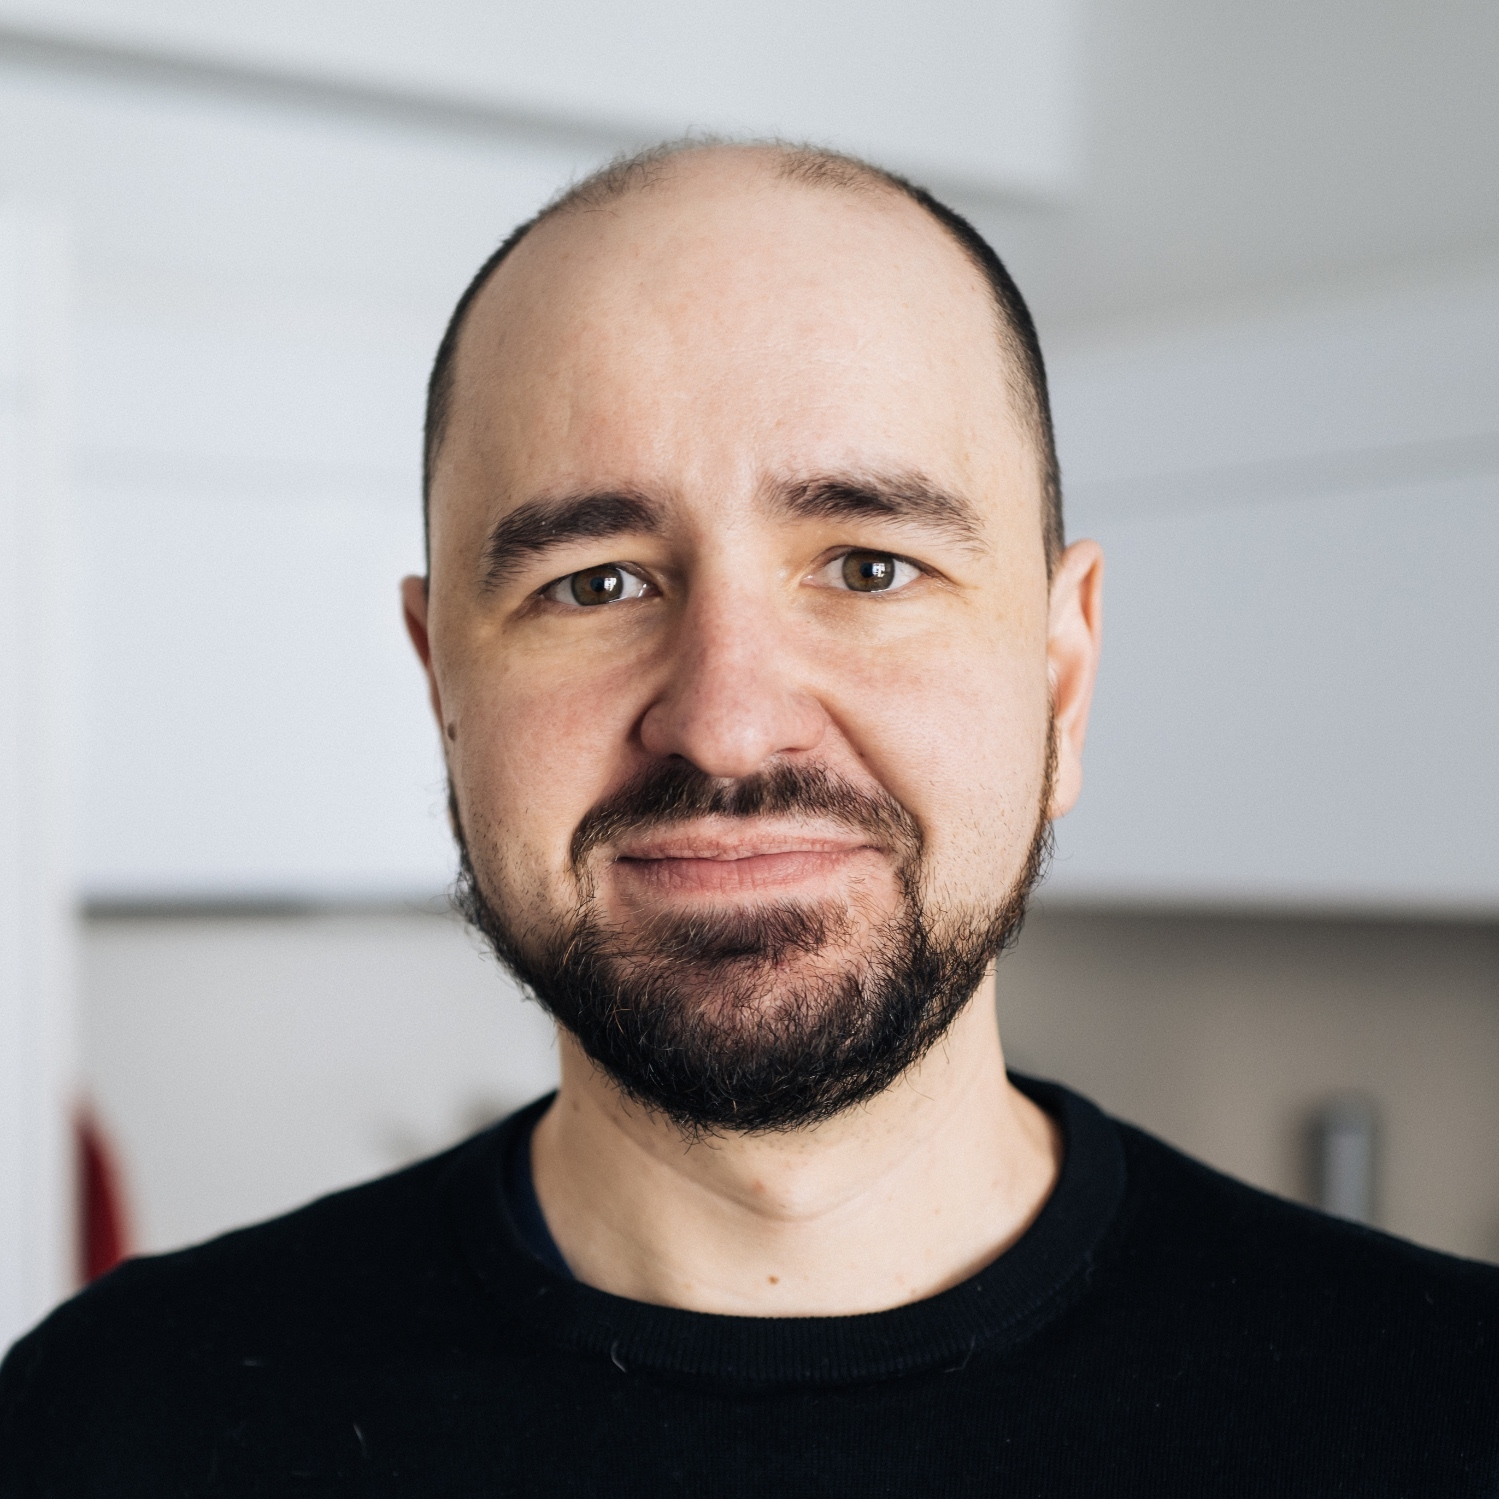
\includegraphics[width=2cm]{myface}};
\end{tikzpicture} \name{\Large Brenden Matthews}
\begin{resume}

\section{Contact} \href{mailto:resume@brenden.brndn.io}{resume@brenden.brndn.io} | \href{https://github.com/brndnmtthws}{github.com/brndnmtthws} | \href{https://brndn.io}{brndn.io}

\vspace{10pt}

\section{Professional Summary}
Visionary software engineer and technical leader with extensive experience in Rust, C, C++, Python, JavaScript, TypeScript, and large-scale infrastructure systems. Recognized expert in Rust programming, with two published books and a prolific open-source portfolio. Proven ability to lead engineering teams, manage cross-functional projects, and deliver transformative technical solutions. Adept at scaling systems, mentoring talent, and fostering a culture of innovation and collaboration.

\vspace{10pt}

\section{Technical Skills}
\begin{itemize}[leftmargin=0.5cm]
    \item \textbf{Programming Languages}: Rust, C, C++, Python, JavaScript, TypeScript, Go, Java, Scala, Bash
    \item \textbf{Cloud \& Infrastructure}: Kubernetes, Docker, Mesos, Nomad, Terraform, AWS, GCP, Azure
    \item \textbf{Data Systems}: Kafka, Cassandra, Snowflake, PostgreSQL, ElasticSearch, Spark, RDS, Redshift, Redis, Hadoop, Presto/Athena
    \item \textbf{Tools \& Libraries}: PyTorch, TensorFlow, Helm, Prometheus, Grafana, Git, Jenkins, CircleCI
    \item \textbf{Methodologies}: Agile Development, Technical Roadmapping, Cross-Functional Leadership, DevOps, CI/CD
\end{itemize}

\vspace{10pt}

\section{Professional Experience}

\textbf{Entrepreneur, Author, Consultant} \hfill \textit{May 2019 -- Present} \\
\textit{New York, NY}
\begin{itemize}[leftmargin=0.5cm]
    \item Founded and scaled multiple businesses, delivering high-quality technical solutions and managing operations end-to-end.
    \item Authored \textit{two best-selling books} on Rust programming, establishing thought leadership in modern software development.
    \item Partnered with global clients as a consultant, providing expertise in cloud migration, Kubernetes adoption, and data engineering.
    \item Developed and launched a Rust-based online coding curriculum, mentoring over 1,000 students.
    \item Created high-impact open-source projects, including:
        \begin{itemize}
            \item \href{https://github.com/brndnmtthws/conky/}{\textbf{Conky}} (7.3k+ stars): Versatile cross-platform system monitor.
            \item \href{https://github.com/brndnmtthws/thetagang/}{\textbf{ThetaGang}} (2k+ stars): Equity options quantitative trading platform leveraging advanced data processing.
            \item \href{https://github.com/brndnmtthws/dryoc/}{\textbf{dryoc}} (280+ stars): Cryptographic library in Rust, offering advanced memory safety features with hard-to-misuse API.
        \end{itemize}
\end{itemize}

\textbf{Braze, Inc.} \hfill \textit{Oct 2018 -- Apr 2019} \\
\textit{Staff Engineer, New York, NY}
\begin{itemize}[leftmargin=0.5cm]
    \item Spearheaded migration of legacy deployment systems to Kubernetes, implementing Helm and Terraform for seamless orchestration.
    \item Designed and rolled out robust CI/CD pipelines, enhancing deployment reliability by 40\%.
    \item Mentored and upskilled a team of 10+ engineers, promoting adoption of modern infrastructure tools and practices.
    \item Defined scalable monitoring strategies using DataDog, achieving 99.9\% uptime for mission-critical services.
\end{itemize}

\textbf{Citadel LLC} \hfill \textit{Oct 2017 -- Jun 2018} \\
\textit{Staff Engineer, New York, NY}
\begin{itemize}[leftmargin=0.5cm]
    \item Architected a modernized, hybrid cloud data platform, integrating on-premises and cloud environments (AWS \& GCP).
    \item Led migration of data systems to PostgreSQL, improving query performance by 60\%.
    \item Guided data science teams in deploying large-scale machine learning models with Spark and Snowflake.
\end{itemize}

\textbf{D2IQ (fka Mesosphere)} \hfill \textit{Jan 2015 -- Feb 2017} \\
\textit{Staff Engineer \& Sales Engineering Lead, San Francisco, CA}
\begin{itemize}[leftmargin=0.5cm]
    \item Built and led the initial sales engineering team, recruiting and training top talent for technical sales and implementation.
    \item Partnered with Fortune 500 clients to define cloud-native transformation strategies, increasing adoption of containerization.
    \item Developed and maintained several frameworks including \textbf{Hadoop}, \textbf{Chronos}, \textbf{Marathon} (and \textbf{marathon-lb}, a critical load balancing tool for DC/OS), and serverless tooling.
\end{itemize}

\textbf{Airbnb, Inc.} \hfill \textit{Feb 2013 -- Jan 2015} \\
\textit{Senior Engineer, Data Infrastructure, San Francisco, CA}
\begin{itemize}[leftmargin=0.5cm]
    \item Pioneered development of scalable data processing pipelines, leveraging Apache Spark, Hadoop, and Mesos.
    \item Played a critical role in creating and scaling \textbf{Apache Superset}, a powerful data visualization platform, and \textbf{Apache Airflow}, a workflow orchestration tool.
    \item Improved organizational data accuracy with an automated verification system, reducing errors and pipeline failures by 90\%.
    \item Improved query times by 100x by optimizing data storage and retrieval mechanisms.
    \item Led a team of 10+ engineers, fostering a culture of innovation and collaboration.
\end{itemize}

\textbf{Newfield Wireless, Inc.} \hfill \textit{Sept 2009 -- Nov 2012} \\
\textit{Senior Software Engineer, Berkeley, CA}
\begin{itemize}[leftmargin=0.5cm]
    \item Developed real-time 3GPP LTE network capture and parsing tools, enhancing data processing efficiency.
    \item Created a custom database solution with an integrated query language, enabling real-time analysis of streaming records.
    \item Designed and implemented communication libraries for high-performance data pipelines in C++ and Python.
\end{itemize}

\textbf{Real Time Measurements, Inc.} \hfill \textit{2003 -- 2009} \\
\textit{Software Engineer, Calgary, AB}
\begin{itemize}[leftmargin=0.5cm]
    \item Built end-user applications, web services, and embedded software for industrial use.
    \item Configured servers and automated IT systems, reducing costs and improving system reliability.
\end{itemize}

\vspace{10pt}

\section{Open Source Contributions}
\begin{itemize}[leftmargin=0.5cm]
\item \textbf{Apache Projects}: Contributed to Apache Kafka, Superset, Airflow, Spark, and Mesos (PMC member).
\item Published and maintained tools with 10k+ combined GitHub stars, reflecting broad adoption and community impact.
\end{itemize}

\vspace{10pt}

\section{Published Works}
\begin{itemize}[leftmargin=0.5cm]
\item \textit{Code Like a Pro in Rust} (Manning Publications) \hfill ISBN: 9781617299643  
\item \textit{Idiomatic Rust: Code like a Rustacean} (Manning Publications) \hfill ISBN: 9781633437463  
\end{itemize}

\vspace{10pt}

\section{Public Speaking}
\begin{itemize}[leftmargin=0.5cm]
\item Delivered talks at \textbf{All Things Open}, \textbf{QCon}, \textbf{LinuxCon}, and other conferences.
\item Frequent keynote speaker on Rust programming, cloud infrastructure, and distributed systems.
\end{itemize}

\end{resume}
\end{document}
